\chapter{Raccolta dati ed implementazione}
\label{chap:implementazione}

Questo capitolo si occuperà, prima di tutto, di fornire dettagli sulle tecnologie e sulle modalità di raccolta dei dati da \textit{Twitter}, necessari alla costruzione di \textit{retweet graphs} associati ad \textit{hashtags} in \textit{input}.
\\Infine verrà trattata puntualmente l'implementazione degli algoritmi, definiti rigorosamente nel capitolo precedente, e di tutte quelle tecniche che hanno permesso di raggiungere l'obiettivo preposto, ovvero l'implementazione di un \textit{framework} che permetta di:
\begin{enumerate}
\item costruire ed analizzare \textit{retweet graphs} associati ad \textit{hashtags di Twitter} in \textit{input};
\item rilevare le \textit{echo-chambers} che caratterizzano la discussione;
\item eseguire un algoritmo di \textit{k-edge recommendation}, in modalità \textit{greedy} o meno;
\item fornire strumenti per l'analisi degli archi consigliati e per la visualizzazione dei nodi coinvolti (i.e. i nodi estremi degli archi consigliati).  
\end{enumerate}

\section{Raccolta dati}
La raccolta dei dati è una fase indispensabile, una condizione \textit{sine qua non}, senza la quale non è pensabile raggiungere alcun obiettivo tra quelli prefissati.
\\Poichè il \textit{software} proposto si occupa di \textit{endorsement graphs} del \textit{social network} di \textit{Twitter}, per la raccolta dei dati si è reso necessario l'utilizzo della \textit{Twitter Api}. Inoltre, visto che il linguaggio utilizzato per l'implementazione è \textit{Python}, sono state sfruttate le funzionalità della libreria \textit{Tweepy}, una via di accesso alla \textit{Twitter Api} di facile utilizzo. 
\\Nel seguito saranno forniti dettagli sugli strumenti di \textit{Twitter Api e Tweepy} e su altre tecniche che hanno permesso di \textit{bypassare} importanti limitazioni temporali delle \textit{Api di Twitter}.  

\subsection{Twitter Api}
\textit{Twitter} mette a disposizione degli sviluppatori delle \textit{Api}, utili per l'acquisizione dei dati pubblicati dagli utenti. Per rendere possibile il loro utilizzo bisogna innanzitutto creare un \textit{account Twitter} e poi effettuare l'iscrizione al \textit{reparto sviluppatori di Twitter}. Questa procedura è molto rigida e qualora non fosse seguita in modo rigoroso non sarebbe possibile utilizzare le \textit{Api}. 
\\Una volta effettuata l'iscrizione al \textit{reparto sviluppatori di Twitter}, è finalmente possibile procedere con la raccolta dei dati pubblicati dagli utenti, ma non prima di aver ottenuto le credenziali di accesso. Le credenziali vengono rilasciate a seguito della creazione di una \textit{Twitter App}, che rappresenta un \textit{progetto Twitter} dello sviluppatore: esse permetteranno di autenticarsi presso un \textit{server di Twitter}, con il quale sarà possibile interagire \textit{via streaming} mediante le \textit{Twitter Api} per ottenere i dati richiesti. Le credenziali si dividono in \textit{Token} e \textit{Consumer}, i quali hanno le seguenti caratteristiche e funzioni:
\begin{itemize}
\item il \textit{Token} permette l'accesso ai servizi che offre \textit{Twitter}. Non è sufficiente per consentire lo \textit{streaming} dei dati dal \textit{server}. \`E costituito da:
\begin{itemize}
\item \textit{Access Token};
\item \textit{Access Secret}.
\end{itemize}
\item il \textit{Consumer} consente lo \textit{streaming} dei dati di \textit{Twitter} dal \textit{server}. \`E costituito da:
\begin{itemize}
\item \textit{Consumer Key};
\item \textit{Consumer Secret}.
\end{itemize}
\end{itemize}
Nell'ambito della stessa \textit{Twitter App}, queste chiavi possono essere rigenerate a piacimento, anche con l'obiettivo di evitare problematiche relavite alla sicurezza. Qualunque sia il linguaggio di programmazione utilizzato per lo sviluppo del \textit{software} (nel caso in esame \textit{Python}), per utilizzare le \textit{Api} da codice è sempre necessario prima autenticarsi, fornendo tutti e quattro i codici appena elencati: le interfacce d'accesso alle \textit{Api} di \textit{Twitter} tuttavia dipendono dal linguaggio di programmazione e, nel nostro caso, sono realizzate mediante la libreria di \textit{Python Tweepy}, della quale parleremo nel seguito della trattazione.
\\Ad ogni modo, bisogna sottolineare che lo \textit{streaming} dei dati viene limitato da \textit{Twitter} per evitare che gli sviluppatori utilizzino in modo sconveniente i dati pubblicati dagli utenti: uno sviluppatore, pur essendo dotato di tutte le credenziali necessarie, non può effettuare più di 100 richieste ogni 15 minuti. Durante il tempo di pausa, che viene fatto scattare in corrispondenza del superamento della soglia di richieste, lo sviluppatore può decidere di aspettare che esso si esaurisca o, al contrario, può decidere deliberatamente di violarlo ed effettuare una nuova richiesta: in tal caso le sue credenziale verrebbero bloccate e non gli sarebbe permesso di comunicare con il \textit{server} mediante le \textit{Api} per circa un'ora.
\\Un'altra limitazione che impone l'\textit{Api} ufficiale di \textit{Twitter} riguarda l'impossibilità di ottenere \textit{tweets} più vecchi di una settimana: questa limitazione è molto forte ed ha costituito, nel processo di sviluppo del \textit{framework} proposto, un problema molto ingente, la cui risoluzione è dovuta alla libreria \textit{GetOldTweets di Python}, della quale parleremo presto.
\\Per terminare, i dati che lo sviluppatore richiede al \textit{server} mediante la \textit{Twitter Api} vengono restituiti in un file \textit{JSON}: esso conterrà tutti i \textit{metadati} necessari, i quali dipendono dal criterio della \textit{query}, come ad esempio il testo del \textit{tweet}, gli \textit{hashtags}, lo \textit{username} dell'utente che l'ha pubblicato e gli utenti che l'hanno \textit{retweettato}.

\subsection{Tweepy}
\textit{Tweepy} è una libreria di \textit{Python} che permette di accedere agevolmente alle \textit{Api} di \textit{Twitter}. Gestisce l'autenticazione dello sviluppatore presso il server di \textit{streaming} utilizzando i seguenti metodi:
\begin{enumerate}
\item \textit{tweepy.OAuthHandler(CONSUMER\_KEY, CONSUMER\_SECRET)}: 
\\una volta forniti \textit{Consumer Key e Consumer Secret} validi, restituisce un codice di autenticazione \textit{auth}; 
\item \textit{auth.set\_access\_token(ACCESS\_TOKEN, ACCESS\_TOKEN\_SECRET)}: 
\\permette di impostare il codice \textit{auth} con gli \textit{Access Token e Access Token Secret} (validi);
\item \textit{tweepy.API(auth)}: restituisce, in caso di corretta autenticazione, un oggetto \textit{Api} attraverso il quale può finalmente avvenire il processo di \textit{streaming} dal \textit{server}.
\end{enumerate}
Inoltre \textit{Tweepy} permette di gestire vari tipi di errore tra cui \textit{RateLimitError}, che insorge quando viene superata la soglia di traffico di 100 richieste ogni 15 minuti.

\subsection{GetOldTweets}
Come precedentemente detto, l'\textit{Api} ufficiale di \textit{Twitter} rende impossibile, con un semplice \textit{account} gratuito, l'acquisizione di \textit{tweets} più vecchi di una settimana. Questa limitazione, nel caso del sistema proposto, è intollerabile, visto che, per costruire \textit{retweet graphs} di dimensioni sufficienti a condurre un'analisi significativa, bisogna utilizzare un intervallo di osservazione abbastanza ampio. Superare tale limitazione continuando ad utilizzare l'\textit{Api} ufficiale vorrebbe dire pagare per ottenere un \textit{account Enterprise}, cosa che non siamo disposti a fare. 
\\La libreria \textit{GetOldTweets} permette di \textit{bypassare} l'\textit{Api} ufficiale e di ottenere \textit{tweets} più vecchi di una settimana semplicemente sfruttando la funzione \textit{scroll} della pagina di \textit{Twitter}: facendo \textit{scroll} verso il fondo pagina è possibile ottenere, tramite chiamate successive ad un \textit{provider JSON}, \textit{tweets} (relativi all'\textit{hashtag} che si sta cercando) via via più vecchi, evitando di incorrere a limitazioni temporali. Tale libreria mette a disposizione un gran numero di criteri di ricerca, utilizzati poi come parametri dell'indirizzo \textit{http}. Nel caso in esame sono stati utilizzati i seguenti parametri:
\begin{itemize}
\item \textit{Since}: una data limite inferiore per limitare la ricerca;
\item \textit{Until}: una data limite superiore per limitare la ricerca;
\item \textit{QuerySearch}: il testo di \textit{query} desiderato. Nel caso in esame, come \textit{query} viene sempre specificato un \textit{hashtag}, il quale identifica una discussione, e vengono considerati tutti e soli i \textit{tweets} creati nell'intervallo temporale specificato e che recano tale \textit{hashtag}.
\end{itemize}
Una volta costruito un oggetto \textit{tweetCriteria}, specificando le informazioni sopra elencate, esso viene passato come parametro al metodo \textit{getTweets} della classe \textit{TweetManager}, il quale si occupa di recuperare tutti i \textit{tweets} che soddisfano i criteri di ricerca. In particolare questo metodo, una volta costruita la \textit{url} contenente tutti i parametri di ricerca specificati, acquisisce la pagina \textit{web} contenente tutti i \textit{tweets} che soddisfano i criteri e converte il risultato in un formato \textit{JSON}. Le informazioni che, nel caso specifico dell'implementazione proposta, vengono estratte dai \textit{tweets} risultanti sono due:
\begin{itemize}
\item \textit{ID} del \textit{tweet};
\item \textit{Username} dell'autore del \textit{tweet}.
\end{itemize}
Gli \textit{ID} dei \textit{tweets} verranno utilizzati per recuperare tutti i \textit{retweets} associati, i quali sono indispensabili per costruire il \textit{retweet graph}.

\subsection{Processo di raccolta dati}
Descritte le caratteristiche e le peculiarità degli strumenti utilizzati per effettuare la raccolta dei dati, ora occorre analizzare il processo che permette di acquisirli e di renderli persistenti. Con tale obiettivo è stata implementata la classe \textit{TwittersRetweets}. Essa fornisce metodi per: 
\begin{enumerate}
\item Specificare i parametri di ricerca (i.e. \textit{Since,Until,QuerySearch}); 
\item Recuperare dal \textit{social network di Twitter} tutti i \textit{tweets} che soddisfano i parametri di ricerca specificati al punto \textit{1.}, insieme agli utenti che li hanno prodotti; 
\item Recuperare tutti i \textit{retweets} che sono stati prodotti verso i \textit{tweets} recuperati al punto \textit{2.};
\item Organizzare i dati ottenuti in un \textit{file} e renderli persistenti.
\end{enumerate}
Un oggetto della classe \textit{TwittersRetweets} ha pertanto i seguenti attributi:
\begin{itemize}
\item \textit{since}, ossia la data di inizio ricerca; 
\item \textit{until}, ossia la data di fine ricerca;
\item \textit{query}, utilizzato, nel caso in esame, per specificare un \textit{hashtag};
\item \textit{twittapi}, ossia l'oggetto \textit{api}, senza il quale è impossibile eseguire lo \textit{streaming}, ottenuto a seguito dell'autenticazione presso un \textit{server} di \textit{Twitter} mediante l'utilizzo della libreria \textit{Tweepy}.
\end{itemize}
Il processo di raccolta dati viene eseguito mediante l'invocazione del metodo \textit{computeRetweets(path)} su un oggetto della classe \textit{TwittersRetweets} che ha come attributi proprio i parametri di ricerca (i.e. \textit{since, until, query}) e l'oggetto \textit{twittapi}.
L'esecuzione del metodo \textit{computeRetweets(path)} si articola in tre fasi, come è possibile evincere dalla figura \ref{fig:raccolta_dati}. Più precisamente:
\begin{enumerate}
\item Il metodo \textit{computeRetweets(path)} innanzittutto si occupa di recuperare tutti i \textit{tweets} che soddisfano i parametri di ricerca e gli utenti che li hanno creati. Per fare questo, viste le limitazioni temporali che impone l'\textit{Api} ufficiale di \textit{Twitter}, si rende necessario l'utilizzo della libreria \textit{GetOldTweets}: vengono specificati i criteri di ricerca dei \textit{tweets} da recuperare ed infine il \textit{TweetManager} si occupa di cercarli nella pagina \textit{html} di \textit{Twitter}, per poi restituirli. I \textit{tweets} restituiti sono caratterizzati da due importanti parametri: \textit{tweetid}, ossia l'identificativo univoco del \textit{tweet}, e lo \textit{username}, ossia l'utente che l'ha emesso. Per mezzo di questi parametri, in questa fase vengono costruiti due oggetti, ossia:
\begin{itemize}
\item \textit{dictioTwitters}: un dizionario che ha come chiavi gli \textit{usernames} degli utenti che hanno emesso i \textit{tweets} recuperati e come valori dei dizionari della forma \textit{\{'tweetcount' : x\}}, dove \textit{x} è il numero dei \textit{tweets} recuperati (e che quindi soddisfano i criteri di ricerca) che sono attribuibili ad un certo \textit{username};
\item \textit{tweetids}: una lista che ha come elementi dei dizionari della forma \textit{\{tweetid : tweetuser\}}, dove \textit{tweetid} identifica un certo \textit{tweet} e \textit{tweetuser} identifica l'utente che l'ha emesso.
\end{itemize}
Questi oggetti vengono opportunamente popolati e poi forniti come \textit{input} alla fase successiva.
\item La fase \textit{2} si occupa di scansionare la lista \textit{tweetids}, restituita dalla fase precedente, per individuare tutti i \textit{retweets} emessi nei confronti dei \textit{tweets} che soddisfano i criteri di ricerca. A fine scansione, questa fase restituisce il dizionario \textit{dictioRetweets}, che ha come chiavi delle tuple del tipo \textit{(retweetuser,tweetuser)}, dove \textit{retweetuser} è lo \textit{username} di un utente che ha \textit{retweettato} almeno un \textit{tweet} emesso dall'utente identificato da \textit{tweetuser}, e come valori dei dizionari del tipo \textit{\{'retweetcount' : x\}}, dove \textit{x} è il numero di volte che l'utente \textit{retweetuser} ha \textit{retweettato} dei contenuti dell'utente \textit{tweetuser}. 
\\Questa volta, tuttavia, tali \textit{retweets} sono ottenuti per mezzo dell'\textit{Api} ufficiale di \textit{Twitter}. In particolare, per ogni elemento \textit{\{tweetid : tweetuser\}} della lista \textit{tweetids}:
\begin{enumerate}
\item mediante l'invocazione del metodo \textit{retweets}, messo a disposizione dalla \textit{Twitter Api}, vengono recuperati tutti i \textit{retweets} emessi nei confronti del \textit{tweet} identificato dal \textit{tweetid}. Tali \textit{retweets} vengono restituiti sotto forma di una lista di \textit{status objects}, un formato particolare che viene gestito dalla \textit{Twitter Api};
\item per ogni \textit{status object}, che corrisponde ad un particolare \textit{retweet}, viene recuperato il \textit{JSON} che lo descrive, da cui viene estratto lo \textit{username} dell'utente che ha effettuato il \textit{retweet} stesso (accedendo opportunamente ai campi del \textit{JSON}), che chiamiamo \textit{retweetuser}. Se la tupla \textit{(retweetuser,tweetuser)} esiste già come chiave nel dizionario \textit{dictioRetweets} allora viene semplicemente aggiornato il valore del campo \textit{'retweetcount'} corrispondente, altrimenti tale tupla viene aggiunta al dizionario come sua nuova chiave con valore \textit{\{'retweetcount' : 1\}}. 
\\Infine, se lo \textit{username} \textit{retweetuser} non è presente come chiave nel dizionario \textit{dictioTwitters}, viene aggiunta la nuova chiave \textit{retweetuser} con valore \textit{\{'tweetcount' : 0\}}, in quanto \textit{retweetuser} non ha mai emesso \textit{tweets} contenenti l'\textit{hashtag} specificato.
\end{enumerate}
Il bloccho di codice che implementa le azioni descritte nei precedenti punti (a) e (b) è opportunamente gestito da una clausola \textit{try}: in effetti, come precedentemente detto, l'invocazione del metodo \textit{retweets} della \textit{Twitter Api}, in caso di superamento della soglia di 100 richieste ogni 15 minuti, potrebbe causare il sollevamento dell'eccezione \textit{tweepy.error.RateLimitError}. Tale eccezione verrebbe gestita nella clausola \textit{except} immediatamente successiva, mettendo in pausa il processo di acquisizione dei \textit{retweets} per 15 minuti, in modo tale da non incorrere al blocco di un'ora delle credenziali;
\item Acquisite le informazioni necessarie alla costruzione del \textit{retweet graph} corrispondente alla \textit{query} (ossia all'\textit{hashtag}) ed all'intervallo temporale \textit{since-until} forniti in input, è possibile procedere con il loro salvataggio in memoria. Infatti, giunto a questa fase, il metodo \textit{computeRetweets(path)} si occupa di rendere persistenti i dati collezionati nel dizionario \textit{dictioRetweets}. Innanzitutto apre il file di testo corrispondente al \textit{path} fornito in input e successivamente, per ogni chiave \textit{key} in \textit{dictioRetweets}, si occupa di salvarvi le informazioni nel formato \textit{"key[0],key[1],retweetcount"}, andando a capo per ogni \textit{entry} inserita. Ricordiamo che \textit{key[0]} è \textit{retweetuser}, \textit{key[1]} è \textit{tweetuser} e \textit{retweetcount} è il numero di volte che \textit{retweetuser} ha \textit{retweettato} \textit{tweets} di \textit{tweetuser}.
\\In figura \ref{fig:retweet_file} è possibile osservare un esempio di tale file di testo.
\\Bisogna sottolineare che questo formato di salvataggio dei dati è stato scelto anche per motivi di compatibilità con lo schema utilizzato dall'articolo \cite{garimella:paper}, in modo tale da poterne riprodurre facilmente i test.
\\\\
\end{enumerate}

\begin{figure}
\begin{center}
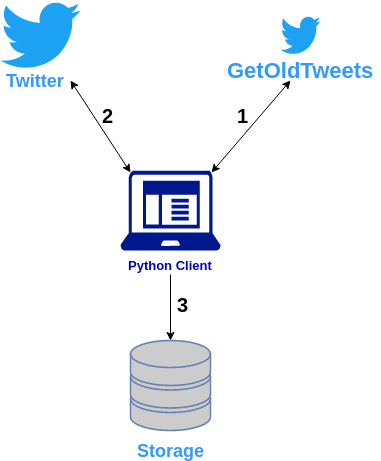
\includegraphics[scale=0.6]{images/raccolta_dati_tesi.png}
\end{center}
\caption{Processo di raccolta dati.}
\label{fig:raccolta_dati}
\end{figure}

\begin{figure}
\begin{center}
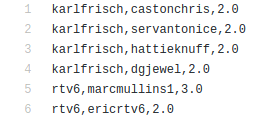
\includegraphics[scale=0.6]{images/retweet_input_file.png}
\end{center}
\caption{Esempio di file che descrive un \textit{retweet graph}.}
\label{fig:retweet_file}
\end{figure}



\section{Implementazione}
